\onecolumn

\begin{figure}
	\begin{minipage}{0.47\textwidth}
		\centering
		
\includegraphics[width=.4\textwidth,left,]{./ETML-ES-LOGO.png}
	\end{minipage}
	
	\hfill
	\begin{minipage}{0.7\textwidth}
		\raggedleft
		\LARGE \textbf{Boîte noire miniaturisée\\ 2023, 1942B}
	\end{minipage}
\end{figure}


% ---- DESCRIPTION ----
\section{Cahier des charges}
\noindent
\begin{minipage}[t]{.5\textwidth} %
	\subsection{Introduction}
	Ce projet vise à stocker les données de mesures et de localisation d'un avion en utilisant une centrale inertielle et un GPS/GNSS. En combinant ces technologies, nous pouvons enregistrer des informations précises sur les caractéristiques du vol et la trajectoire de l'avion. En cas d'accident, ces enregistrements permettent de déterminer les causes potentielles. En somme, ce système de collecte et de stockage de données fournit une compréhension approfondie des vols et des données essentielles. Le cahier des charges détaillé est disponible en annexe.
\end{minipage} %
\begin{minipage}[t]{.5\textwidth} %
	\raggedleft
	\subsection{Aperçu}
	\begin{itemize}
		\item[•]	Sauvegarde des données inertielles chaque 500ms par défaut.
		\item[•]	Sauvegarde des données de localisation chaque 5'000ms par défaut.
		\item[•]	Possibilité de configurer les temps de sauvegarde.
		\item[•]	Résistance aux chocs.
		\item[•]	Bonne autonomie / Low power.
		\item[•]	\Gls{gps}
		\item[•]	\Gls{gnss}.
		\item[•]	\Gls{timestamp} par satellite.
		\item[•]	\gls{centrale inertielle} :
		\subitem- 	Accéléromètre 3-axes. 
		\subitem-	Gyroscope 3-axes.
		\item[•] Charge, lecture et config. par USB-C.
	\end{itemize}
\end{minipage}

% ---- TACHES ----
\subsection{Tâches à réaliser}
Développement et intégration d’un PCB avec capteurs et logging sur carte SD dans un boitier compact.
\begin{itemize}
	\item[•] Développement schématique 
	\subitem- Fonctionnement MCU.
	\subitem-	Périphériques de mesures et de sauvegarde / Bus de communication.
	\subitem-	Gestion batterie 
	\item[•]	Routage pour intégration dans boitier résistant aux chocs.
	\item[•]	Programmation mesure et sauvegarde des données.
	\subitem-	Configuration MCU.
	\subitem-	Configuration du périphérique de mesure pour \gls{imu}.
	\subitem-	Configuration du périphérique de sauvegarde (Carte SD).
	\subitem-	Configuration du périphérique de localisation \gls{gps}/\gls{gnss}.
	\subitem-	Configuration et communication avec l'interface.
	\subitem-	Communication et traitement des données mesurées.
\end{itemize}

\subsection{Schéma de principe}
% ---- SChema de principe ----
\begin{figure}[h]
	\centering
	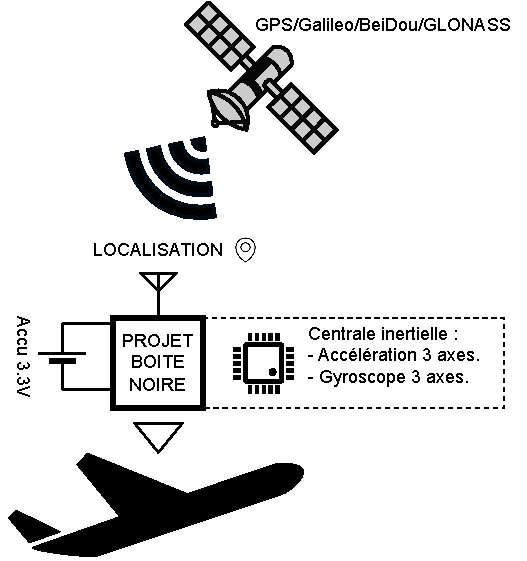
\includegraphics[width=0.6\linewidth]{../figures/cdc/schema_principe}
	\caption{Schéma de principe.}
	\source{Auteur}
	\label{fig:schemaprincipe}
\end{figure}

Ce système électronique de mini boîte noire pour avion, serait capable d'enregistrer des informations récentes sur les données inertielle et la position d'un vol, dans une mémoire non volatile (carte microSD). Le dispositif, abrité dans un boîtier plastique pour assurer une réception optimale des données \gls{gps} et une installation compact. Celui-ci fournirait des données via un port USB pour l'extraction des mesures sur la carte microSD ou pour configurer des paramètres tels que les intervalles de mesures. Les mesures sur les trois axes d'accélération et de vitesse angulaire seraient recueillies par défaut toutes les 500 ms et les données de position \gls{gps} toutes les 5000 ms. Des intervalles d'enregistrement plus longs sont envisageables pour optimiser la durée de vie de la carte SD, selon la taille et l'organisation des données. Le dispositif sauvegarderait les données des 15 dernières minutes de vol (ou plus) dans un fichier CSV pour traitement ultérieur, selon le principe FIFO. L'objectif principal du prototype est de privilégier la compacité pour minimiser son encombrement à bord de l'avion.


\clearpage

% ---- JALONS ----
\subsection{Planification}
\begin{figure}[h]
	\centering
	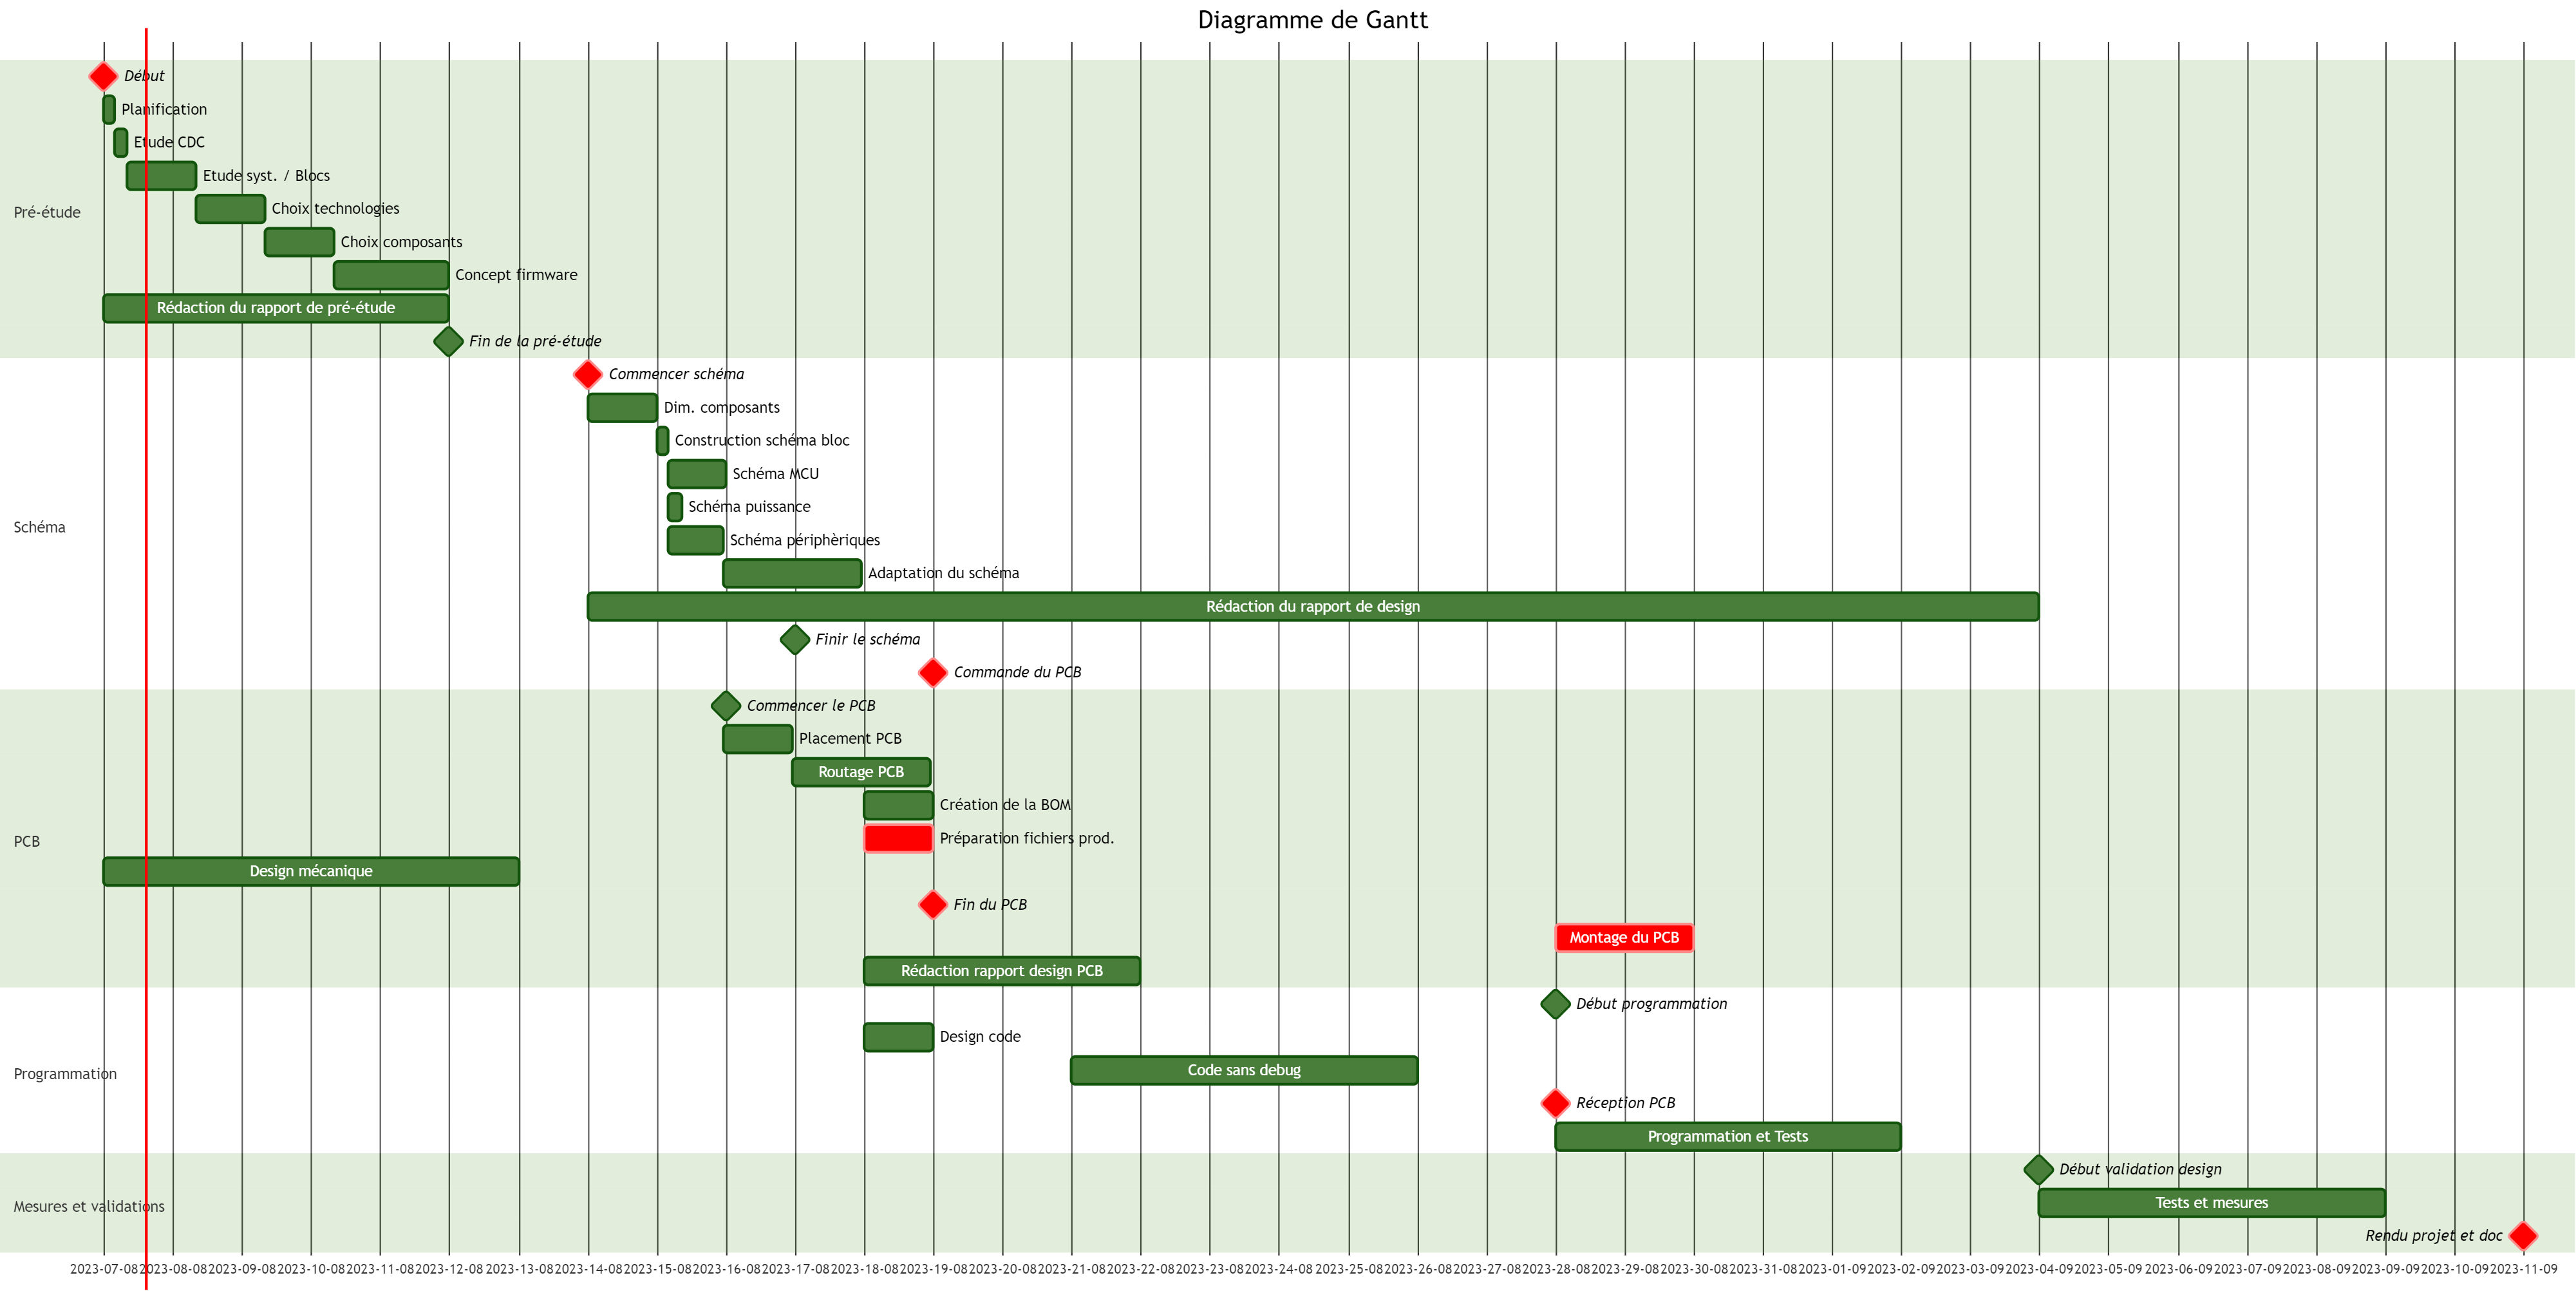
\includegraphics[width=1\linewidth]{../figures/cdc/planif}
	\caption{Planification, Diagramme de gantt.}
	\source{Auteur}
	\label{fig:planification}
\end{figure}
\begin{figure}[h]
	\centering
	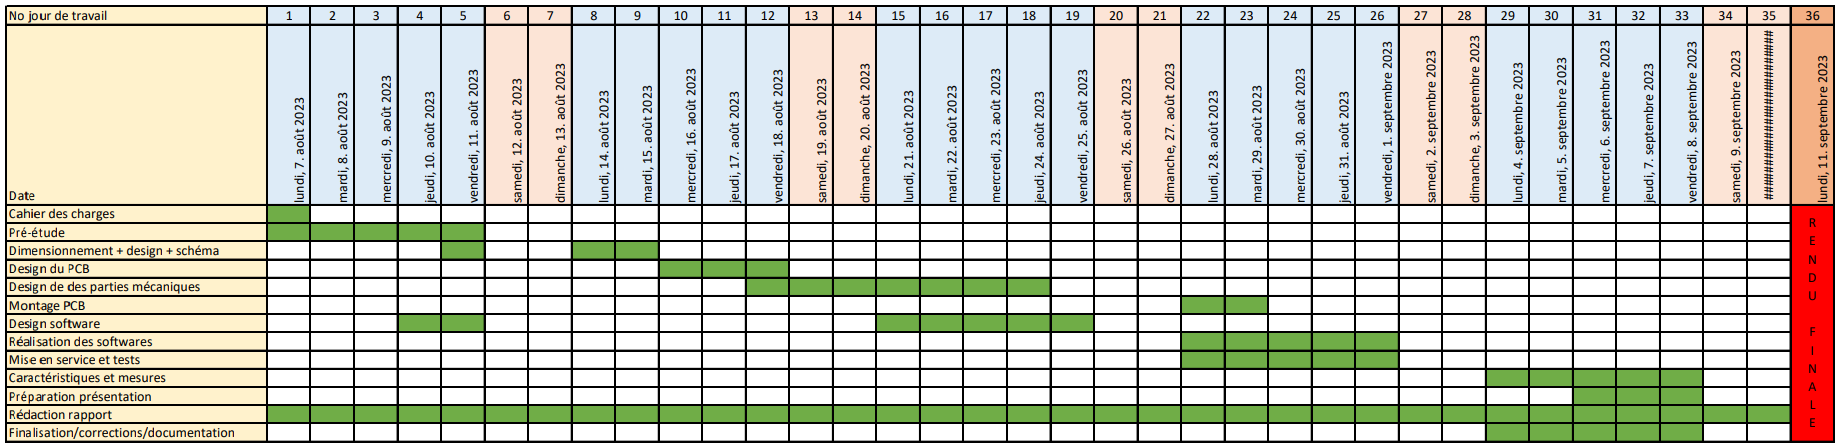
\includegraphics[width=1\linewidth]{../figures/cdc/planif_theorique}
	\caption{Planification théorique.}
	\source{Auteur}
	\label{fig:planiftheorique}
\end{figure}


\subsection{Livrable}
\begin{itemize}
	\item[•] Les fichiers sources de CAO électronique des PCB réalisés
	\item[•] Tout le nécessaire à fabriquer un exemplaire hardware de chaque :
	\item[•] fichiers de fabrication (GERBER) / liste de pièces avec références pour commande / implantation
	\item[•] Prototype fonctionnel
	\item[•] Modifications / dessins mécaniques, etc
	\item[•] Les fichiers sources de programmation microcontrôleur (.c  / .h)
	\item[•] Tout le nécessaire pour programmer les microcontrôleurs (logiciel ou fichier .hex)
	\item[•] Un calcul / estimation des coûts
	\item[•] Un rapport contenant les calculs - dimensionnement de composants - structogramme, etc.
\end{itemize}

\clearpage
